\documentclass[a4paper,12pt,twoside]{memoir}

% Castellano
\usepackage[spanish,es-tabla]{babel}
\selectlanguage{spanish}
\usepackage[utf8]{inputenc}
\usepackage[T1]{fontenc}
\usepackage{lmodern} % Scalable font
\usepackage{microtype}
\usepackage{placeins}
%\usepackage{listings}
%\usepackage{pdflscape}

\RequirePackage{booktabs}
\RequirePackage[table]{xcolor}
\RequirePackage{xtab}
\RequirePackage{multirow}

% Links
\usepackage[colorlinks]{hyperref}
\hypersetup{
	allcolors = {red}
}

% Ecuaciones
\usepackage{amsmath}

% Rutas de fichero / paquete
\newcommand{\ruta}[1]{{\sffamily #1}}

% Párrafos
\nonzeroparskip


% Imagenes
\usepackage{graphicx}
\newcommand{\imagen}[2]{
	\begin{figure}[!h]
		\centering
		\includegraphics[width=1\textwidth]{#1}
		\caption{#2}\label{fig:#1}
	\end{figure}
	\FloatBarrier
}

\newcommand{\imagenflotante}[2]{
	\begin{figure}%[!h]
		\centering
		\includegraphics[width=0.9\textwidth]{#1}
		\caption{#2}\label{fig:#1}
	\end{figure}
}



% El comando \figura nos permite insertar figuras comodamente, y utilizando
% siempre el mismo formato. Los parametros son:
% 1 -> Porcentaje del ancho de página que ocupará la figura (de 0 a 1)
% 2 --> Fichero de la imagen
% 3 --> Texto a pie de imagen
% 4 --> Etiqueta (label) para referencias
% 5 --> Opciones que queramos pasarle al \includegraphics
% 6 --> Opciones de posicionamiento a pasarle a \begin{figure}
\newcommand{\figuraConPosicion}[6]{%
  \setlength{\anchoFloat}{#1\textwidth}%
  \addtolength{\anchoFloat}{-4\fboxsep}%
  \setlength{\anchoFigura}{\anchoFloat}%
  \begin{figure}[#6]
    \begin{center}%
      \Ovalbox{%
        \begin{minipage}{\anchoFloat}%
          \begin{center}%
            \includegraphics[width=\anchoFigura,#5]{#2}%
            \caption{#3}%
            \label{#4}%
          \end{center}%
        \end{minipage}
      }%
    \end{center}%
  \end{figure}%
}

%
% Comando para incluir imágenes en formato apaisado (sin marco).
\newcommand{\figuraApaisadaSinMarco}[5]{%
  \begin{figure}%
    \begin{center}%
    \includegraphics[angle=90,height=#1\textheight,#5]{#2}%
    \caption{#3}%
    \label{#4}%
    \end{center}%
  \end{figure}%
}
% Para las tablas
\newcommand{\otoprule}{\midrule [\heavyrulewidth]}
%
% Nuevo comando para tablas pequeñas (menos de una página).
\newcommand{\tablaSmall}[5]{%
 \begin{table}
  \begin{center}
   \rowcolors {2}{gray!35}{}
   \begin{tabular}{#2}
    \toprule
    #4
    \otoprule
    #5
    \bottomrule
   \end{tabular}
   \caption{#1}
   \label{tabla:#3}
  \end{center}
 \end{table}
}

%
% Nuevo comando para tablas pequeñas (menos de una página).
\newcommand{\tablaSmallSinColores}[5]{%
 \begin{table}[H]
  \begin{center}
   \begin{tabular}{#2}
    \toprule
    #4
    \otoprule
    #5
    \bottomrule
   \end{tabular}
   \caption{#1}
   \label{tabla:#3}
  \end{center}
 \end{table}
}

\newcommand{\tablaApaisadaSmall}[5]{%
\begin{landscape}
  \begin{table}
   \begin{center}
    \rowcolors {2}{gray!35}{}
    \begin{tabular}{#2}
     \toprule
     #4
     \otoprule
     #5
     \bottomrule
    \end{tabular}
    \caption{#1}
    \label{tabla:#3}
   \end{center}
  \end{table}
\end{landscape}
}

%
% Nuevo comando para tablas grandes con cabecera y filas alternas coloreadas en gris.
\newcommand{\tabla}[6]{%
  \begin{center}
    \tablefirsthead{
      \toprule
      #5
      \otoprule
    }
    \tablehead{
      \multicolumn{#3}{l}{\small\sl continúa desde la página anterior}\\
      \toprule
      #5
      \otoprule
    }
    \tabletail{
      \hline
      \multicolumn{#3}{r}{\small\sl continúa en la página siguiente}\\
    }
    \tablelasttail{
      \hline
    }
    \bottomcaption{#1}
    \rowcolors {2}{gray!35}{}
    \begin{xtabular}{#2}
      #6
      \bottomrule
    \end{xtabular}
    \label{tabla:#4}
  \end{center}
}

%
% Nuevo comando para tablas grandes con cabecera.
\newcommand{\tablaSinColores}[6]{%
  \begin{center}
    \tablefirsthead{
      \toprule
      #5
      \otoprule
    }
    \tablehead{
      \multicolumn{#3}{l}{\small\sl continúa desde la página anterior}\\
      \toprule
      #5
      \otoprule
    }
    \tabletail{
      \hline
      \multicolumn{#3}{r}{\small\sl continúa en la página siguiente}\\
    }
    \tablelasttail{
      \hline
    }
    \bottomcaption{#1}
    \begin{xtabular}{#2}
      #6
      \bottomrule
    \end{xtabular}
    \label{tabla:#4}
  \end{center}
}

%
% Nuevo comando para tablas grandes sin cabecera.
\newcommand{\tablaSinCabecera}[5]{%
  \begin{center}
    \tablefirsthead{
      \toprule
    }
    \tablehead{
      \multicolumn{#3}{l}{\small\sl continúa desde la página anterior}\\
      \hline
    }
    \tabletail{
      \hline
      \multicolumn{#3}{r}{\small\sl continúa en la página siguiente}\\
    }
    \tablelasttail{
      \hline
    }
    \bottomcaption{#1}
  \begin{xtabular}{#2}
    #5
   \bottomrule
  \end{xtabular}
  \label{tabla:#4}
  \end{center}
}



\definecolor{cgoLight}{HTML}{EEEEEE}
\definecolor{cgoExtralight}{HTML}{FFFFFF}

%
% Nuevo comando para tablas grandes sin cabecera.
\newcommand{\tablaSinCabeceraConBandas}[5]{%
  \begin{center}
    \tablefirsthead{
      \toprule
    }
    \tablehead{
      \multicolumn{#3}{l}{\small\sl continúa desde la página anterior}\\
      \hline
    }
    \tabletail{
      \hline
      \multicolumn{#3}{r}{\small\sl continúa en la página siguiente}\\
    }
    \tablelasttail{
      \hline
    }
    \bottomcaption{#1}
    \rowcolors[]{1}{cgoExtralight}{cgoLight}

  \begin{xtabular}{#2}
    #5
   \bottomrule
  \end{xtabular}
  \label{tabla:#4}
  \end{center}
}


















\graphicspath{ {./img/} }

% Capítulos
\chapterstyle{bianchi}
\newcommand{\capitulo}[2]{
	\setcounter{chapter}{#1}
	\setcounter{section}{0}
	\chapter*{#2}
	\addcontentsline{toc}{chapter}{#2}
	\markboth{#2}{#2}
}

% Apéndices
\renewcommand{\appendixname}{Apéndice}
\renewcommand*\cftappendixname{\appendixname}

\newcommand{\apendice}[1]{
	%\renewcommand{\thechapter}{A}
	\chapter{#1}
}

\renewcommand*\cftappendixname{\appendixname\ }

% Formato de portada
\makeatletter
\usepackage{xcolor}
\newcommand{\tutor}[1]{\def\@tutor{#1}}
\newcommand{\course}[1]{\def\@course{#1}}
\definecolor{cpardoBox}{HTML}{E6E6FF}
\def\maketitle{
  \null
  \thispagestyle{empty}
  % Cabecera ----------------
\noindent
\includegraphics[width=\textwidth]{cabecera}\vspace{1cm}%
  \vfill
  % Título proyecto y escudo informática ----------------
  \colorbox{cpardoBox}{%
    \begin{minipage}{.8\textwidth}
      \vspace{.5cm}\Large
      \begin{center}
      \textbf{TFG del Grado en Ingeniería Informática}\vspace{.6cm}\\
      \textbf{\LARGE\@title{}}
      \end{center}
      \vspace{.2cm}
    \end{minipage}

  }%
  \hfill\begin{minipage}{.20\textwidth}
    
\includegraphics[width=\textwidth]{escudoInfor}
  \end{minipage}
  \vfill
  % Datos de alumno, curso y tutores ------------------
  \begin{center}%
  {%
    \noindent\LARGE
    Presentado por \@author{}\\ 
    en Universidad de Burgos --- \@date{}\\
    Tutor: \@tutor{}\\
  }%
  \end{center}%
  \null
  \cleardoublepage
  }
\makeatother

\newcommand{\nombre}{Alejandro Fernández Lampreave} %%% cambio de comando

% Datos de portada
\title{Generación de rutas utilizando sistemas empotrados}
\author{\nombre}
\tutor{Dr. Alejandro Merino Gómez}
\date{\today}

\begin{document}

\maketitle


\newpage\null\thispagestyle{empty}


%%%%%%%%%%%%%%%%%%%%%%%%%%%%%%%%%%%%%%%%%%%%%%%%%%%%%%%%%%%%%%%%%%%%%%%%%%%%%%%%%%%%%%%%
\thispagestyle{empty}


\noindent
\includegraphics[width=\textwidth]{cabecera}\vspace{1cm}

\noindent D. Alejandro Merino Gómez, profesor del departamento de Ingeniería Electromecánica, área de Ingeniería de Sistemas y Automática.

\noindent Expone:

\noindent Que el alumno D. \nombre, con DNI 71290315K, ha realizado el Trabajo final de Grado en Ingeniería Informática titulado Generación de rutas utilizando sistemas empotrados. 

\noindent Y que dicho trabajo ha sido realizado por el alumno bajo la dirección del que suscribe, en virtud de lo cual se autoriza su presentación y defensa.

\begin{center} %\large
En Burgos, {\large \today}
\end{center}

\vfill\vfill\vfill

% Author and supervisor
%\begin{minipage}{0.45\textwidth}
%\begin{flushleft} %\large
%Vº. Bº. del Tutor:\\[2cm]
%D. nombre tutor%
%\end{flushleft}
%\end{minipage}
%\hfill
%\begin{minipage}{0.45\textwidth}
%\begin{flushleft} %\large
%Vº. Bº. del co-tutor:\\[2cm]
%D. nombre co-tutor
%\end{flushleft}
%\end{minipage}
%\hfill

%\vfill

% para casos con solo un tutor comentar lo anterior
% y descomentar lo siguiente
Vº. Bº. del Tutor:\\[2cm]
D. Alejandro Merino Gómez


\newpage\null\thispagestyle{empty}




\frontmatter

% Abstract en castellano
\renewcommand*\abstractname{Resumen}
\begin{abstract}
Este proyecto se centra en utilizar la placa de desarrollo FRDM K64F, con un módulo GPS incorporado, que sea capaz de registrar en una tarjeta microSD la ruta seguida por el dispositivo. La información recogida por el dispositivo será mostrada en una interfaz web.
 
Para ello se debe desentramar la cadena GPS y almacenarla. La activación/desactivación de la captura GPS se hará de acuerdo a la información recogida por el acelerómetro.
\end{abstract}

\renewcommand*\abstractname{Descriptores}
\begin{abstract}
Generación de rutas, módulo GPS, aceleróemtro, sistema empotrado, registro microSD, estadísticas diarias, aplicación web.
\end{abstract}

\clearpage

% Abstract en inglés
\renewcommand*\abstractname{Abstract}
\begin{abstract}
This project focuses on using the FRDM K64F development board, with a built-in GPS module, which is capable of recording the path followed by the device on a microSD card. The information collected by the device will be displayed in a web interface.
 
To do this, the GPS chain must be unlocked and stored. The activation / deactivation of the GPS capture will be done according to the information collected by the accelerometer.
\end{abstract}

\renewcommand*\abstractname{Keywords}
\begin{abstract}
Routes generation, GPS module, accelerometer, embedded system, microSD log, daily statistics, web application.
\end{abstract}

\clearpage

% Indices
\tableofcontents

\clearpage

\listoffigures

\clearpage

%\listoftables
\clearpage

\mainmatter
\capitulo{1}{Introducción}


El proyecto se centra en la generación de rutas a través de un sistema embebido mediante la recolección de datos que aporta el módulo GPS adherido a la placa. Este desarrollo busca crear una herramienta que recolecte y almacene las coordenadas GPS y represente en un mapa la ruta generada. De esta manera se permite una visualización completa de todos los puntos almacenados y un histórico de los datos recogidos en diferentes días.


\section{Estructura de la memoria}

\begin{itemize}
\tightlist
\item
    \textbf{Objetivos del proyecto}: plantea los objetivos que se pretenden solucionar.
\item
    \textbf{Conceptos Teóricos}: exposición de las diferentes cuestiones teóricas vistas durante el proyecto.
\item
    \textbf{Técnicas y herramientas}: listado de las diferentes técnicas y herramientas utilizadas a lo largo del proyecto.
\item
    \textbf{Aspectos relevantes del desarrollo del proyecto}: muestra los aspectos con más relevancia en la realización del proyecto.
\item
    \textbf{Trabajos relacionados}: muestra algunos trabajos con cierto grado de similitud a la generación de rutas.
\item
    \textbf{Conclusiones y líneas de trabajo futuras}: conclusiones obtenidas en la realización del proyecto y algunas posibles ideas futuras de mejora.
\end{itemize}

\section{Estructura de los anexos}

\begin{itemize}
\tightlist
\item
    \textbf{Plan de Proyecto Software}: planificación temporal y estudio de la viabilidad legal y económica.
\item
    \textbf{Especificación de requisitos}: expone los requisitos y objetivos establecidos al principio del desarrollo.
\item
    \textbf{Especificación de diseño}: recoge la información del diseño arquitectónico y el procedimental.
\item
    \textbf{Manual del programador}: incluye los aspectos más importantes para el programador: cómo instalar las herramientas, compilar, instalar y ejecutar.
\item
    \textbf{Manual de usuario}: guía de información básica para el usuario, para un uso correcto de la aplicación.
\end{itemize}

\capitulo{2}{Objetivos del proyecto}

En este capítulo trataremos de abordar cuáles han sido los objetivos estipulados en el proyecto que denominaremos objetivos generales y también nombraremos como objetivos técnicos aquellos que vienen dados a la hora de llevar a cabo los anteriores.

\section{Objetivos generales}
\begin{itemize}
\tightlist
\item
    Almacenar las coordenadas suministradas por el GPS en la tarjeta microSD. 
\item
	Desarrollar una web que muestre la ruta almacenada.
\item
    Poder almacenar los datos en archivos de texto a modo de histórico.
\item
    Poder descargar una imagen del mapa con la ruta.
\end{itemize}

\clearpage

\section{Objetivos técnicos}
\begin{itemize}
\tightlist
\item
	Cablear los pines Tx y Rx tanto de envío como de recepción de datos del módulo GPS con los pines digitales I/O, 0 y 1 del mismo.
\item
	Desentramar la cadena GPS transmitida por el módulo GPS, adherido a la placa de desarrollo.
\item
	Enviar los datos del módulo GPS en modo soft serial a través del puerto (UART3) y por puerto serie (UART0) al ordenador.
\item
	Guardar los mensajes NMEA recibidos en la tarjeta microSD.
\item
	Incluir un sistema operativo de tiempo real (RTOS) para la gestión de los procesos.
\item
    Desarrollar una interfaz web intuitiva y clara para el usuario que permita la subida de ficheros.
\item
	Los archivos deberán ser convertidos de NMEA a GeoJSON.
\item
	Los ficheros se guardarán en el servidor acompañados de la fecha y hora.
\item
    La ventana de la interfaz debe adaptarse a diferentes tamaños y resoluciones de pantalla.
\item
    La aplicación podrá utilizarse en cualquier dispositivo con un navegador instalado.
\item
    La aplicación deberá representar las coordenadas recogidas en el menor tiempo posible.
\item
    Emplear Git como herramienta de control de versiones incluido en la plataforma GitHub.
\end{itemize}


\capitulo{3}{Conceptos teóricos}

Inicialmente, uno de los apartados que más dificultad presentaba el proyecto era que tendría que manejarme con un estándar de posicionamiento y se tendría que realizar sobre un sistema embebido, nunca antes había trabajado con uno. A continuación se detallan algunos de los conceptos más importantes que ayudarán a la comprensión del proyecto.

\section{Sistema embebido}
Se denomina \textit{Sistema embebido} \cite{embebido} a aquel sistema electrónico que está diseñado para un propósito específico. Suelen ser compactos, realizan tareas sencillas y tienen todos o la mayoría de componentes que necesitan para desarrollar su función incorporados.

Las características de un \textit{Sistema embebido} son \cite{embebido2}:
\begin{itemize}
\tightlist
\item
	Deben ser sistemas robustos.
\item
	Deben ser sistemas confiables, es decir que trabaje correctamente (reliability).
\item
	Después de un fallo deben volver a funcionar en un periodo corto de tiempo (maintainability).
\item 
	Deben estar disponibles en cualquier momento (availability).
\item 
	La comunicación ha de ser confidencial y autentificada.
\item 
	Son eficientes desde un punto de vista energético, de peso, de coste y de cantidad de código.	
\item 
	Habitualmente nos les encontramos sin teclado, ratón ni pantalla.
\end{itemize}

\section{Sistema de Posicionamiento Global GPS}
Entendemos por \textit{GPS} \cite{GPS}, como un sistema de posicionamiento global de radionavegación, con origen en Los Estados Unidos de América. Ofrece gratuitamente posicionamiento, navegación y cronometría de forma ininterrumpida a toda la tierra y sin número límite de usuarios. Solo es necesario contar con un receptor GPS, el sistema te proporcionará tu localización y hora local, independientemente de las condiciones climáticas y tu posición.

A día de hoy el \textit{GPS} se ha convertido en una herramienta imprescindible en todos los medios de transporte, ya sea tierra mar o aire y es utilizado a diario por los servicios de emergencia a la hora de localizar, coordinar y socorrer.
Además, se ha convertido en los últimos años, en un elemento de vital importancia en operaciones bancarias o en las redes energéticas, entre otras, ya que se gana precisión cronométrica.

\section{Estándar NMEA}
NMEA \cite{NMEA} corresponde a la abreviatura National Marine Electronics Association es una asociación creada por un grupo de marcas relacionadas con la electrónica naval, a la que de forma progresiva se fueron adhiriendo más grupos y colectivos oficiales. \cite{NMEA2}

En la versión de NMEA0183 ya existían GPS enviando información a través de este protocolo, sin embargo, solo estaba diseñado para enviar o recibir una señal y en ningún caso era capaz de recibir dos señales distintas. Para tal efecto se ayudaba de lo que se conoce como un distribuidor NMEA, cuya función es la de recibir las señales de cada dispositivo, procesarlas, y emitir una nueva señal con la información en una misma cadena.

Con la nueva versión NMEA 2000, podemos prescindir de este distribuidor ya que soporta la conexión de diferentes equipos enviando y recibiendo información simultáneamente.

El propósito del estándar NMEA a día de hoy principalmente reside en dar un mismo soporte común a una gran variedad de GPS, en lugar de que cada uno tenga que desarrollar el suyo propio. Lo que incrementa la dificultad del estándar es que no hay solo una cadena con información, hay varias con distintos propósitos que, aunque no siempre se aprovechan todas.

Vamos a poner un ejemplo de una de las cadenas más frecuentes en NMEA: \cite{NMEA3}.
\$GPGGA,172009.00,4205.7041778,N,09054.4977280,W,4,14,1.00,394.123,M,
28.199,M,0.10,0000*39

Todas las cadenas empiezan por \$ y los campos van separados por comas.

\begin{itemize}
\tightlist
\item
    GP: representa que se trata de una posición GPS.
\item
    172009.00: hora, 17:20:09 UTC.
\item
    4205.7041778: latitud.
\item
    N: punto cardinal de la latitud, Norte.
\item
	09054.4977280: longitud.
\item
	W: punto cardinal de la longitud, Oeste. 
\item
	4: precisión de la coordenada (mín 1-4 max).
\item
	14: número de satélites usados.
\item
	1.00: Dispersión de la precisión horizontal o incertidumbre (HDOP).
\item
	394.123: altura de la antena.
\item
	M: unidad de medida de la altura de la antena.
\item
	28.199: altura geoidal (restando la altura de la antena obtenemos la altura elipsoidal HAE).
\item
	M: unidad usada en la altura geoidal.
\item
	0.10: segundos desde la última actualización (opcional).
\item
	0000: ID de la estación (opcional).
\item
	*39: checksum.
\end{itemize}

Aparte del mensaje NMEA \$GPGGA hay otros frecuentemente utilizados como \$GPGLL y \$GPRMC que son muy similares y también incluyen las coordenadas. Pero hay otros menos utilizados capaces de aportar diferente información que no detallaremos por no sernos de utilidad. Como por ejemplo \$GPGSA, \$GPGSV, \$GPVTG o \$GPGST.

\section{Sistema operativo de tiempo real para sistemas empotrados}
Hablamos de sistema operativo de tiempo real \cite{tiemporeal} o RTOS cuando la importancia no recae sobre los usuarios si no sobre los procesos, de forma que se le exige dar una respuesta en un tiempo previamente determinado, si no, diremos que ha fallado. Los RTOS disponen de mecanismos de comunicación, sincronización, acceso a recursos compartidos y sincronización. Destacan: FreeRTOS, MQx y VxWorks.

Algunas de sus características son \cite{tiemporeal_c}:
\begin{itemize}
\tightlist
\item
	El uso de memoria es más bien escaso.
\item
	Un evento en el hardware puede ejecutar una tarea.
\item
	El código sirve para múltiples arquitecturas de CPU.
\item
	Usualmente poseen tiempos de respuesta predecibles.
\end{itemize}

\subsection{FreeRTOS}
FreeRTOS \cite{FreeRTOS} es uno de los sistemas operativos de tiempo real existentes, apto para al menos 35 plataformas de microcontrolador diferentes. Una de sus principales ventajas reside en que se encuentra distribuida bajo la licencia gratuita y de libre uso MIT \cite{MIT}.

Está escrito en C, para facilitar su legibilidad, portabilidad y mantenibilidad. 
Diseñado para ser simple y pequeño, lo que facilita su utilización en sistemas empotrados, consta de métodos para la creación de hilos (con prioridades), semáforos, temporizadores etc. Las tareas se ejecutan en función de la prioridad y se van rotando por medio de una interrupción.

\section{CRS}
La función de un sistema de coordenadas de referencia\cite{crs} es definir, junto con la ayuda de las coordenadas, la forma en la que un mapa bidimensional se relaciona con lugares reales de la tierra. Este mapa bidimensional será proyectado en un GIS. (programa informático que se utiliza para relacionar datos geográficos).
Los CRS pueden dividirse en sistemas de referencia de coordenadas geográficos o proyectados.
El sistema de coordenadas geográficas utiliza los grados de longitud, latitud y en ocasiones altitud para representar la situación.
La latitud se representa tomando como referencia la línea del ecuador y se divide a cada hemisferio en 90 secciones.
La longitud se basa en el meridiano de Greenwich y son líneas perpendiculares al ecuador.
El sistema de referencia de coordenadas proyectado normalmente se define en un plano bidimensional denominado plano XY. X será el eje horizontal e Y el eje vertical. 
En ocasiones se añade un tercer eje, el Z, por lo que el sistema se definirá en un plano tridimensional.

\section{EPSG}
Acrónimo de European Pretoleum Survey Group,\cite{epsg} es una organización que se relaciona con la industria del petróleo en Europa. Este organismo desarrolló un archivo de parámetros geodésicos que contiene información sobre las proyecciones cartográficas de todo el mundo.
En la actualidad, las tareas del EPSG las lleva a cabo el Subcomité de Geodesia del Comité de Geomática de la OGP.
Este archivo es de gran importancia ya que es utilizado para la definición de datos de posición en los Sistemas de Información Geográfica. Será de gran utilidad para las actividades que requieran trabajar con datos espaciales en un ambiente digital.

\section{UART}
Universal Asynchronous Receiver-Transmitter.\cite{uart} Se trata de un bus serie muy usado en microcontroladores, encargado de recibir y transmitir información de forma asíncrona entre ordenadores y otros microcontroladores. Es posible su utilización a través de software en caso necesario. Es en el caso concreto de los ordenadores donde se utilizan los “puerto serie” o COM. La velocidad de transmisión con la que se envía y recibe información, es expresada en baudios y mide la cantidad de datos (bits) que se envían en un segundo. Actualmente está siendo sustituido por otras comunicaciones como la SATA o USB, sin embargo, persiste en la industria.

\section{I2C}
Acrónimo de Inter-Integrated Circuit.\cite{i2c} Estándar de comunicación creado en un principio por Philips para las televisiones, ahora destaca por su implementación en la conexión entre microcontroladores o con periféricos.

\section{SPI}
Serial Peripheral Interface. \cite{spi} Otro estándar de comunicación creado por Motorola, en este caso periféricos con comunicación en serie y síncronos. Tiene la peculiaridad de que permite la conexión uno a varios (maestro-esclavos) a través de Full Duplex.

\section{Tarjeta microSD}
También conocida como TransFlash,\cite{tarjeta} fue creada por SanDisk en el 2005 con el objetivo de almacenar información digital incorporándolas en diferentes sistemas. Trabajan a 3.3V, apenas llegan a los 15 milímetros en su parte más alargada, pero sin embargo, pueden llegar alcanzar capacidades de 2TB. Actualmente se pueden adquirir tarjetas de diferentes tamaños velocidades y capacidades. Como desventaja remarcar que no disponen de ningún sistema de protección contra escritura.

\section{Acelerémetro}
Un acelerómetro\cite{acelerometro} es una herramienta encargada de medir vibraciones o bien la aceleración que experimenta un cuerpo. La fuerza que se genera con el movimiento ejerce una presión sobre un material piezoeléctrico, que a su vez produce una diferencia de potencial que puede ser expresada en fuerzas G. La carga es directamente proporcional a la aceleración debido a que la masa no varía y depende directamente de la fuerza experimentada(F=m.a).

\capitulo{4}{Técnicas y herramientas}

\section{Kinetis}
Para conseguir almacenar los mensajes NMEA en la tarjeta microSD, se ha utilizado Kinetis Design Studio 3 IDE \cite{kinetis}. Se trata de un software de desarrollo basado en GNU/Eclipse antes utilizado en exclusiva para los servicios de los dispositivos de Freescale Kinetis. Desde la adquisición por parte de NXP ahora presta servicio a multitud de sistemas empotrados.

Soporta dispositivos Kinetis basados en Cortex-M, integra Processor Expert y un kit de desarrollo de software. 
Además soporta diversas herramientas de debugueo, entre ellas: SEGGER J-Link/J-Trace, P\&E USB Multilink Universal/USB Multilink Universal FX y CMSIS-DAP. Utiliza la nueva librería nano C que ayuda a reducir la memoria utilizada por el sistema embebido.

\section{Lenguaje C}
El lenguaje C \cite{C} es un lenguaje de programación poco tipificado, de tipo de datos estático y de medio nivel porque tiene las estructuras comunes de los de alto nivel, pero además también tiene estructuras que le habilitan un control a bajo nivel.

Cuenta como principal virtud la eficiencia que su código produce. Normalmente utilizado en la creación de software de sistemas y ciertas aplicaciones. La programación a bajo nivel permite la modificación de registros del procesador, lo que lo convierte en ideal para la programación de sistemas empotrados.

\section{Processor Expert}
Processor Expert \cite{ProcessorExpert} es un sistema de desarrollo para configurar, crear, optimizar y migrar componentes software para las placas de desarrollo. 
Los componentes embebidos propios de las placas de desarrollo, son módulos que puedes instalar con Processor Expert  y que vienen con una serie de funcionalidades incorporadas especialmente diseñadas para sacar el máximo partido a dicho componente. Cobra un papel muy importante en nuestro proyecto dado que la programación directa de sistemas empotrados es compleja. Se trata de una programación a muy bajo nivel que requiere el acceso y la modificación de registros o incluso llegando a la programación en ensamblador. Con la intención de evitar esto, nace esta herramienta que proporciona una serie de librerías que permiten la programación a más alto nivel.

Cuando lo usamos genera dependiendo del componente, cabeceras, ciertos archivos de configuración o código fuente.

Un componente representa un elemento hardware, un periférico, un algoritmo o cualquier colección lógica de funciones.
\begin{figure}[!h]
	\centering
	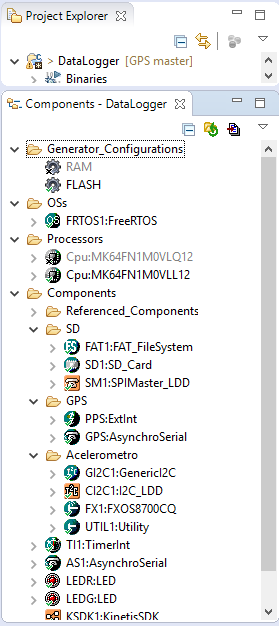
\includegraphics[width=0.5\textwidth]{ProcessorExpert.PNG}
	\caption{Processor Expert, vista de los diferentes componentes instalados.}\label{fig:ProcessorExpert.PNG}
\end{figure}
\FloatBarrier

\section{Termite}
Termite \cite{termite} es una terminal que permite la comunicación serie entre pc y placa, haciendo uso de los puertos COM del ordenador. Cuenta con una interfaz similar a la de un chat, en la que va mostrando toda la información que recibe y además cuenta con una línea para poder introducir texto y poder enviarlo.

\imagen{termite.PNG}{Terminal termite, ventana en blanco donde imprime la información que recibe.}

\section{Mapbox}
Mapbox \cite{mapbox} es un proveedor de mapas online para páginas web que nació en 2010. Se utiliza para integrar mapas en aplicaciones móviles y web.
Es una de las plataformas de datos más elegidas por los clientes por diferentes aspectos.
En Mapbox todo es personalizable, puedes escoger cualquier color, ocultar la capa que no quieras del mapa, etc. Tiene una serie de estilos predefinidos, pero también puedes crear el tuyo a través de la herramienta MapboxStudio.
Todo su código es open source y puedes encontrarlo en GitHub, lo que te permite ver las funcionalidades que están en desarrollo, notificar cualquier problema, hasta puedes contribuir mandando mejoras.
Se puede utilizar en cualquier plataforma, ya que hay SDKs disponibles para la mayoría, Android, iOS, web, etc.

\section{MyGeodata}
Mygeodata \cite{mygeodata} es un conversor de datos geográficos en línea que consta de diferentes formatos, CAD, GIS y Raster.

Se divide en tres apartados principales aunque en el proyecto solo se ha aprovechado el conversor:
\begin{itemize}
\tightlist
\item
	\textit{Drive}: en el cual puedes guardar tu conjunto de datos y gestionarlos o ver archivos que hayan compartido otros usuarios.
\item
	\textit{Converter}: es el apartado online donde puedes traducir tus coordenadas al formato de datos que elijas.
\item
	\textit{Map}: donde se muestran nuestros datos en un mapa de forma online.	
\end{itemize}

\section{XAMPP}
XAMPP \cite{xampp} es una herramienta que permite realizar pruebas de nuestro trabajo en el ordenador sin la necesidad de tener acceso a internet. Es una forma sencilla de instalar Apache.
Cuenta con un intérprete del lenguaje PHP, servidores de bases de datos como MySQL, servidores FTP, etc.
Su instalación es muy sencilla, basta con descargar y ejecutar un archivo comprimido, con unas pequeñas configuraciones. Además se actualiza de forma regular para que el usuario tenga las últimas versiones de los diferentes servidores que tiene.

\section{PHP}
PHP \cite{php} es un lenguaje \textit{open source} y puede ser incrustado en HTML.
Se ejecuta en el servidor web, por lo que puede tener acceso a bases de datos, conexiones de red y otra serie de tareas para crear la página resultado que será la que vea el cliente. Esta página final contendrá únicamente código HTML, por lo que será compatible con cualquier navegador.
Que el lenguaje se combine con HTML hace que sea fácil de utilizar, una de sus grandes ventajas, además de ser gratuito, multiplataforma, tenga una gran seguridad y rapidez.
Fue creado por Ramus Lerdorf en 1994, pero al ser de código abierto ha tenido varias contribuciones a lo largo de estos años.

\section{Python}
Python \cite{python} es un lenguaje orientado a objetos, que puede utilizarse para distintos objetivos, desde aplicaciones Windows a páginas web. Es muy conocido por varias razones, tiene una gran cantidad de librerías que cuentan con funciones muy útiles, es sencillo y rápido en comparación a otros lenguajes, se puede desarrollar en varias plataformas y es gratuito.
Fue creado por Guido Van Rossum, cuyo objetivo era un lenguaje que hiciese más fácil la orientación a objetos.
Las características más destacables del lenguaje son:
\begin{itemize}
\tightlist
\item
	Es de propósito general, puede utilizarse para la creación de varios programas.
\item
	Es multiplataforma, existen diferentes versiones para sistemas informáticos distintos.
\item
	Interpretado, no hay que compilar el código para realizar la ejecución. Es verdad que sí hay una compilación, pero es transparente al programador.
\item
	Es interactivo, podemos ejecutar cada sentencia para ver qué nos muestra.
\item
	Es un lenguaje orientado a objetos.
\item
	Cuenta con una gran cantidad de funciones y librerías que hacen más sencillo el trabajo, evitando tener que programar desde cero.
\item
	La sintaxis utilizada es muy sencilla y clara, se utiliza la tabulación para separar el código y distinguir los bucles o funciones.
	
\end{itemize}
Todo esto hace que Python actualmente esté siendo utilizado en empresas como Google, Yahoo, la NASA, etc

\section{GitHub}
GitHub \cite{GitHub} es una plataforma online de desarrollo colaborativo de software para almacenar en la nube proyectos, haciendo uso del sistema de control de versiones Git.
Git es un sistema de control de versiones de código abierto, gratuito y distribuido. Ha sido creado para poder manejar cualquier proyecto con eficiencia y velocidad. Github ha sido utilizado en este proyecto como piedra angular, para tener en todo momento el control sobre las distintas versiones.

\section{ZenHub}
ZenHub \cite{ZenHub} es una extensión que puede integrarse en GitHub, pero contiene interfaz propia.
Con ella nos ayudamos a tener un mayor control sobre nuestros proyectos, con un sistema de paneles, donde podemos ir catalogando las diferentes tareas según la fase de desarrollo en la que se encuentren. 

Los diferentes segmentos o \textit{pipelines} en los que se puede encontrar una tarea o \textit{issue} son: \textit{New issues, Icebox, Backlog, In progress Review/QA, Done y Closed} pero se pueden añadir más.

Además genera estadísticas, tiene un sistema de votación y permite obtener retroalimentación. Su gran baza al igual que GitHub, es que es gratuito para proyectos públicos. 

\section{LaTeX}
LaTeX \cite{latex} es un sistema utilizado para componer textos, principalmente indicado para aquellos que necesiten de una alta calidad de acabado tipográfico. Para la creación de esta memoria se ha utilizado Texmaker \cite{texmaker}.

\subsection{MiKTeX}
Además, junto con junto Texmaker hemos necesitado MiKTeX \cite{miktex} de código abierto, tiene compiladores LaTex y TeX y tiene la posibilidad de instalar unos 800 paquetes diferentes con macros, tipografías etc.

\section{Sonarcloud}
Sonarcloud\cite{sonarcloud} consiste en una plataforma \textit{online} que nos permite evaluar la calidad del código de nuestro proyecto de forma gratuita. Utiliza herramientas avanzadas que le permiten detectar posibles fallos o vulnerabilidades y que nos pueden ayudar a mejorar nuestro código. De forma general te presentan un panel informativo tras analizar el código con los siguientes aspectos: \textit{Bugs, vulnerabilities, code smells, coverage y duplications}. Se aporta el link del proyecto para poder revisarlo.

\section{Selenium}
Selenium\cite{selenium} es una herramienta que permite realizar pruebas de código sobre proyectos web. En nuestro caso se han llevado a cabo con Selenium IDE que ofrece una interfaz que permite grabar nuestros movimientos dentro de la web y provee una serie de comandos para hacer \textit{asserts} de una forma mas intuitiva que con Selenium WebDriver. De forma adicional permite exportar los test creados. 


\capitulo{5}{Aspectos relevantes del desarrollo del proyecto}

%Debe incluir desde la exposición del ciclo de vida utilizado, hasta los detalles de mayor relevancia de las fases de análisis, diseño e implementación.
%Se busca que no sea una mera operación de copiar y pegar diagramas y extractos del código fuente, sino que realmente se justifiquen los caminos de solución que se han tomado, especialmente aquellos que no sean triviales.
%Puede ser el lugar más adecuado para documentar los aspectos más interesantes del diseño y de la implementación, con un mayor hincapié en aspectos tales como el tipo de arquitectura elegido, los índices de las tablas de la base de datos, normalización y desnormalización, distribución en ficheros3, reglas de negocio dentro de las bases de datos (EDVHV GH GDWRV DFWLYDV), aspectos de desarrollo relacionados con el WWW...
%Este apartado, debe convertirse en el resumen de la experiencia práctica del proyecto, y por sí mismo justifica que la memoria se convierta en un documento útil, fuente de referencia para los autores, los tutores y futuros alumnos.

Este capítulo trata de recoger los aspectos más interesantes del desarrollo del proyecto. Las diferentes decisiones que se tomaron, pasando por los múltiples problemas que se sucedieron, propios de un proyecto creado desde cero y cómo se fueron solventando.

%\label{sec:ciclodevida}
\section{Ciclo de vida del desarrollo}       
El proyecto ha ido desarrollándose y se ha distribuido de forma semanal, basándonos en la metodología ágil Scrum. De forma que cada semana había una reunión con el tutor, en las que se veía el estado del proyecto y se establecían las nuevas tareas.

Lo primero fue instalar el entorno de desarrollo, una vez configurado y con el sistema embebido en mi poder, me puse manos a la obra y fui viendo cómo funcionaba la placa, el módulo gps y el IDE. Una vez hechas las conexiones del módulo gps, para que pudieran pasar los datos a la placa, se pudo ver por primera vez gracias a un pequeño código, cómo se mostraban los mensajes NMEA por pantalla, en la terminal de Termite. 
\imagen{conexiones.PNG}{Conexiones hechas entre los pines Rx y Tx hacia Digital I/O 1 y 0 respectivamente.}

El siguiente paso fue ver cómo funcionaba el acelerómetro que incorporaba la placa, para ello se decidió hacer un programa que almacenase los datos recogidos por él mismo en la tarjeta microSD. 

Para ello, se necesitaban crear y configurar diferentes módulos para que pudiesen funcionar, nos hemos basado en unos tutoriales que, a pesar de estar en algunos casos desactualizados, nos han servido de base \cite{tutorial}. Algunos de estos módulos fueron: 
\begin{itemize}
\tightlist
\item
	El sistema de almacenamiento.
\item
	El componente del acelerómetro.
\item
	El componente de la unidad de tiempo.	
\item
	El componente de la fecha.
\item
	El componente de secciones críticas.
\item
	El componente de la tarjeta microSD.
\item
	El componente de la comunicación síncrona.
\end{itemize}
Cabe destacar que la mayoría de estas interfaces necesitan una pequeña configuración en sus parámetros para que sean funcionales y se terminen de acoplar con el resto del sistema, no entraremos en detalle ya que considero que se escapa del objetivo de esta memoria, sin embargo queda citado por si fuera de interés\cite{tutorial}.
Finalmente, tras esto y una pequeña función, teníamos los datos del acelerómetro en la tarjeta microSD. 

Era el momento hacer lo mismo con los mensajes NMEA proporcionados por el módulo GPS, pero antes había que instalar dos módulos más\cite{tutorial2}, el de una interrupción externa y el de una señal asíncrona que sería la encargada de pasar los datos del módulo GPS a la placa. De esta forma ya podíamos almacenar las coordenadas en un archivo de texto.
\imagen{placa.PNG}{Placa de desarrollo FRDMK64F con el módulo GPS integrado y registrando datos.}

A continuación vendría la creación de la interfaz para poder mostrar las coordenadas, previamente almacenadas.
Se hizo una primera versión de una interfaz que simplemente mostrara un mapa donde poder representar coordenadas, para ello nos ayudamos de una API como es Mapbox. En este punto del proyecto se consiguió representar por primera vez una ruta. Sin embargo debía automatizar el proceso ya que la conversión de los datos arrojados por la placa (NMEA) y los leídos por la API de Mapbox había sido realizada de forma manual, mediante una herramienta de internet. 

El primer paso consistía en transformar los datos de NMEA a GeoJSON de forma automática, para ello, fue imprescindible la ayuda de la API de MyGeodata, realizando un script en Python que se encargaba de ello.
A partir de ahí vino la implementación de la subida de archivos al servidor, para así poder pasárselo al convertidor. Una vez que el archivo estaba almacenado en la carpeta \textit{subidas}, ya se podía convertir, descomprimir los archivos generados y representarlos en el mapa. 

Mas tarde se añadieron algunas funcionalidades al mapa como los controles de navegación, edificios tridimensionales, la opción de descargar una imagen del mapa, centrarlo basándose en tu localización o la de regresar a la página de inicio. Además se añadieron las excepciones al código.

Por último se contó con herramientas como Selenium o Sonarcloud para hacer las pruebas del sistema y comprobar la calidad del código respectivamente.

El resultado del proyecto se compone de todas estas fases de desarrollo por las que ha ido pasando. A continuación abordaremos de una forma más detallada todos los problemas técnicos que surgieron, cómo los tratamos y sobre todo cómo fueron resueltos, con mayor o menor acierto.

\section{Resoluciones técnicas}

\subsection{Arreglar Kinetis Studio}
Tras apenas una semana de trabajo sobre el proyecto, Kinetis Design Studio dejó de funcionar, para ser más exactos, la carga de Processor Expert al ser integrado en un nuevo proyecto bloqueaba el programa quedando cargando en el 4\%.

Lo primero que se hizo fue probar con otros proyectos, pero no importaba si era nuevo o ya estaba creado, si contenía Processor Expert no cargaba correctamente. Se comprobó el log de errores que arrojaba y tras mucho buscar por internet no se encontró una solución válida, se optó por borrar registros, parámetros, re-instalaciones parciales del Processor Expert e incluso reinstalar el programa entero en varias ocasiones. 

Tras ver que nada de esto funcionaba se optó por limpiar el registro de Windows, lo cual tampoco lo solventó. Por último solo se pudo pensar en una restauración del sistema operativo, que finalmente sí tuvo éxito.

\subsection{Almacenar los valores del acelerómetro en la tarejeta microSD} 
Como un primer acercamiento a los componentes de la placa tras haber realizado la Práctica 1 de Sistemas Empotrados en el que se creaba un \textit{Hola mundo}, se opta por capturar los datos aportados por los ejes del acelerómetro y almacenarlos en la tarjeta microSD. Se ha llevado a cabo con unas líneas de código que luego podremos tomar como referencia para enviar las coordenadas del GPS por puerto serie.
\imagen{ejes.PNG}{Acelerómetro de 6 ejes.\cite{ejes}}

\subsubsection{Añadir componentes básicos}
Una vez creado el proyecto y con la configuración básica debemos añadir algunos componentes. En este caso, para poder almacenar la información en la tarjeta utilizaremos el componente \textit{Fat\_FileSystem} que permite almacenar los datos gracias a la función FAT1\_Write. 
Pero este componente requiere otro que aporte la fecha, para ello elegimos \textit{GenericTimeDate} y por último, uno que permita proteger las secciones críticas (\textit{CriticalSection})), necesario para evitar que una interrupción pueda hacer que la fecha que se proporcione sea inconsistente. Las secciones críticas evitan que una interrupción o tarea de más prioridad haga un cambio de contexto dentro de la misma.

Además se requiere implementar una comunicación serie síncrona de tipo maestro esclavo, de la cual se encarga el componente SPIMaster\_LDD, donde solo dos dispositivos se pueden comunicar entre si al mismo tiempo.
\begin{figure}[!h]
	\centering
	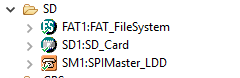
\includegraphics[width=0.5\textwidth]{sd.PNG}
	\caption{Componentes necesarios para permitir el almacenamiento el la tarjeta microSD.}\label{fig:sd.PNG}
\end{figure}
\FloatBarrier

Hay que relacionar y configurar todos los componentes (como por ejemplo \textit{SPIMaster\_LDD} estableciendo cuales serán los pines de entrada y salida de datos de la placa con el pc).

Para poder trabajar con el acelerómetro es necesario añadir también \textit{FXOS8700CQ} que contiene varias funciones entre las que destacan, FX1\_GetX(), FX1\_GetY() y FX1\_GetZ(). Se encargan de obtener los valores de cada eje en ese preciso momento.
Automáticamente se añadirá el componente \textit{GenericI2C} que implementa un \textit{driver} genérico para el bus de comunicaciones en serie I2C (Inter\-Integrated Circuit), de esta forma funciona tanto para controladores de dispositivos lógicos \textit{LDD} (Logical Device Driver) como para los clásicos que no lo son. En nuestro caso particular nos interesa activar la comunicación LDD I2C y esto obliga a añadir un componente más \textit{I2C\_LDD} que encapsula la interfaz de la comunicación I2C.
\begin{figure}[!h]
	\centering
	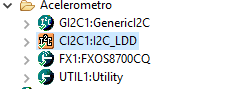
\includegraphics[width=0.5\textwidth]{acelerometro.PNG}
	\caption{Componentes para poder obtener los datos del acelerómetro.}\label{fig:acelerometro.PNG}
\end{figure}
\FloatBarrier

Por último tuve que comprobar que detectaba la tarjeta microSD y que se encontraba montado y funcionando el archivo del sistema (\textit{fileSystemObject}).

\subsection{Mostrar las sentencias NMEA por pantalla}
Para recoger la información del módulo GPS debemos saber que una vez que el módulo conecta con los satélites, produce un \textit{PPS (Pulso por Segundo)} cada 100 milisegundos.
Por lo tanto, lo primero que debemos hacer es añadir los módulos necesarios y configurar los parámetros según el tutorial que me sirvió de guía \cite{tutorial2}. Primero el módulo \textit{ExtInt}, que no es más que una señal externa que se sincroniza con los pulsos del GPS, de forma que así podemos contar los pulsos o simplemente sincronizarlos con otras señales propias.

Segundo, necesitamos AsynchroSerial \textit{AsynchroSerial} una señal asíncrona que implementa el protocolo serie UART y que interactuará con las líneas Rx y Tx del GPS. Como el receptor está constantemente enviando la información con 9600 baudios, debemos seleccionar la misma tasa.
\begin{figure}[!h]
	\centering
	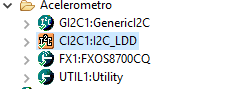
\includegraphics[width=0.5\textwidth]{acelerometro.PNG}
	\caption{Componentes necesarios del módulo GPS.}\label{fig:gps.PNG}
\end{figure}
\FloatBarrier

Ahora con los módulos añadidos y configurados quedaba añadir el código que permitiera la visualización de las sentencias NMEA a través de la terminal Termite. Con esto era suficiente, pero como veremos en el siguiente punto, al añadir \textit{FreeRTOS} se incorpora una cadena de caracteres donde almacenar las sentencia NMEA y un manejador de la misma \textit{(xQueueHandle)}.

\imagen{imprime.PNG}{Función Imprime encargada de pasar los datos al pc por puerto serie.}

\subsection{Almacenar las sentencias NMEA en la tarjeta microSD}
Ahora que ya tenemos la configuración hecha (de las coordenadas del acelerómetro), que permite el almacenamiento de datos en la tarjeta SD, parece obvio que tan solo fuera necesario reutilizar la cadena ya rellenada con nuestra información, pero aquí vino una de las mayores dificultades, se perdía información muy probablemente porque antes de que acabara de escribir en la cadena se empezaba a escribir en la tarjeta microSD y viceversa, de forma que se optó por incluir un sistema operativo en tiempo real como \textit{FreeRTOS}. Para ello tuve que documentarme, añadir dos módulos necesarios al proyecto para que funcionara, \textit{FreeRTOS} y \textit{KinetisSDK}, y crear las tareas pertinentes con su nivel de prioridad asociado. De esta forma, ahora la información que se muestra en la pantalla se pasa directamente a la función \textit{EscribeSD()} encargada de escribir una cadena dada, en la tarjeta microSD.

Como medida de eficiencia se optó por únicamente almacenar los mensajes NMEA de tipo GPRMC, que aportan toda la información que nosotros necesitamos reduciendo en un 75\% la cantidad de datos almacenados.

Los datos se introducen en la cadena con el método \textit{xQueueSendToBack} (dado que es una cola FIFO) y se extraen con \textit{xQueueReceive} por el final de la cola. 
\imagen{chargps.PNG}{Tarea en tiempo real dedicada a recibir e introducir los caracteres en la cadena.}

De manera adicional se decidió dar utilidad al diodo led rgb que incorpora la placa y se configuró de forma que emitiera luz verde (\textit{LEDR\_Off()y LEDG\_Neg()})cuando estuviera recolectando datos del GPS y luz roja(\textit{LEDR\_Neg()y LEDG\_Off()}) cuando estuviera ocupado escribiendo en la tarjeta microSD.
\imagen{escribeSD.PNG}{Código necesario para el correcto envío de datos a la tarjeta microSD.}

\subsection{Añadir un sistema en tiempo real}
En un principio cabe destacar que no incluimos un sistema operativo de tiempo real, lo cual generaba diferentes problemas, el principal es que era necesario programar la gestión y planificación de las tareas, utilizando hilos, interrupciones periódicas etc. Esto cuando el problema es sencillo se puede hacer, pero cuando el problema empieza a complicarse es mejor delegarlo en un RTOS. 

En consecuencia, la información almacenada no correspondía en muchas ocasiones con la mostrada por pantalla. 
Más adelante descubrimos que esto se debía a que muy probablemente estuviéramos almacenando información en nuestra cadena antes si quiera de llegar a escribir por completo la que ya teníamos en el buffer. Utilizamos FreeRTOS por ser uno de los más extendidos para pequeños sistemas embebidos. Añadimos el módulo correspondiente en Kinetis \textit{FreeRTOS} y lo configuramos.
\imagen{tareas.PNG}{Inicialización de tareas de tiempo real.}

\subsection{Elección de la API para representar las rutas}
Puede parecer un tema trivial, pero se le dio bastante importancia. En un primer momento siempre se consideró la opción de utilizar la de Google Maps, de hecho se llegó a realizar el código para que funcionara (y así lo hizo), pero desde junio de 2018 se convirtió en una API de pago, si bien te otorgan en tu cuenta de Google Maps, 300\$ al mes de crédito para gastar en su API en función del tráfico que tengan tus mapas creados, había que introducir una forma de pago por si excedías el límite, por lo que no me pareció la mejor de las opciones.
\begin{figure}[!h]
	\centering
	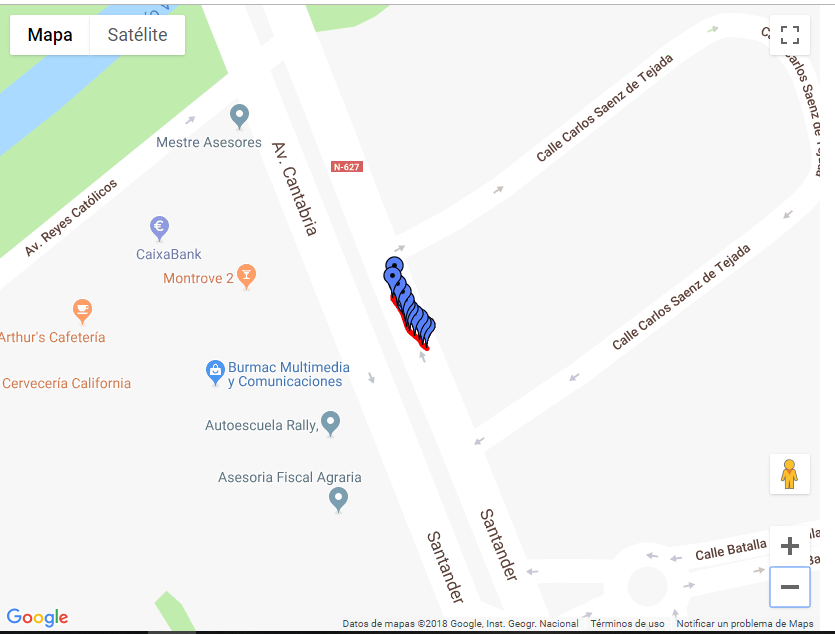
\includegraphics[width=0.7\textwidth]{google.PNG}
	\caption{Mapa creado con la API de Google.}\label{fig:google.PNG}
\end{figure}
\FloatBarrier

De forma que busqué una alternativa gratuita, es ahí donde descubrí Mapbox, una API que poco tiene que envidiar de la de Google. Con un funcionamiento similar multitud de opciones y gratuita. Ya cuenta con numerosas empresas que usan sus servicios como: Tinder, Bosch, National Geographic, Mastercard, CNN o Snapchat entre las más importantes.
\imagen{empresas.PNG}{Empresas que ya trabajan con Mapbox.}

\subsection{Creación de una interfaz básica HTML}
Con la ayuda de la documentación de Mapbox\cite{mapboxapi} se creó una primera página HTML sencilla que mostraba unas coordenadas pasadas directamente en un array. Pensé que tendría que leer las que yo había capturado de forma aislada y pasárselas. Por fortuna descubrí que se podía pasar el fichero entero en formato GeoJSON. Convertí mi archivo NMEA a GeoJSON con una herramienta web y pasándoselo o bien de manera local o un enlace raw de GitHub funcionaba perfectamente. Pero el objetivo era automatizar este proceso y que la mayoría de acciones fueran transparentes al usuario.
\begin{figure}[!h]
	\centering
	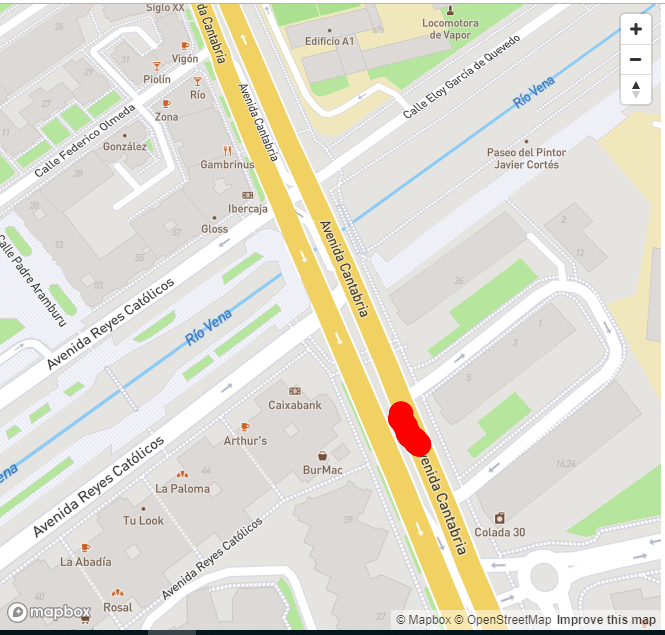
\includegraphics[width=0.7\textwidth]{mapboxgeojson.PNG}
	\caption{Mapa creado con la API de Mapbox.}\label{fig:mapboxgeojson.PNG}
\end{figure}
\FloatBarrier

\subsection{Conversión automática de NMEA a GeoJSON}
Tras mucho investigar descubrí que la conversión de NMEA a GeoJSON es una de las menos frecuentes, son más típicas otras como GPX (para el caso del receptor Garmin) o KML en el caso de querer representar en Google Maps. Estuve barajando hacer un parser manualmente, pero tendría que dedicar muchos recursos en aprender las espeficaciones del estándar GeoJSON, así que por temas de eficiencia opté por buscar un recurso que lo agilizara. Descubrí MyGeodata, que es sin ninguna duda el mejor sitio web para convertir entre cientos de estándares. Solo había un problema y era que de forma gratuita solo ofrece 3 conversiones mensuales, pero tras hablar con el soporte y explicar mi situación de estudiante, me ofrecieron una \textit{key} gratuita. 

Con la ayuda de su documentación,\cite{mygeodataapi} desarrollé el código, pero entre los parámetros que había que poner para poder hacer uso de su herramienta se encontraba uno que me estaba dando problemas. Se trata de \textit{outcrs}, (sistema de referencias de coordenadas de salida) que no sabía qué había que indicar, más allá del formato de salida que se deseaba. Por defecto se realiza mediante \textit{'EPSG:3857'}, necesario para conversiones para la API de Google en KML, en nuestro caso Mapbox necesitaba GeoJSON de forma que nos correspondía \textit{'EPSG:4326'}.
\imagen{outcrs.PNG}{Información básica que necesita para poder convertir el archivo.}

\subsection{Habilitar la subida de archivos al servidor}
La opción más cómoda y amigable que se me ocurrió para el usuario, con la que estuviera familiarizado, fue que realizara la subida del archivo tal cual lo encontraba en la microSD. La parte del \textit{backend} se encargaba de convertirlo y cargarlo, con la opción que brinda en un futuro tener los archivos en el servidor para poder mostrar el mapa deseado por el usuario.
 
La subida se hace mediante un formulario que llama al archivo \textit{upload\_file.php} que es el encargado de casi todo. En un principio se representaba el mapa en la página principal, pero al no tener todavía las coordenadas y estar vacío se decidió mover a una página secundaria con el fin de optimizar la página de inicio.
\imagen{upload.PNG}{Formulario que habilita la subida de archivos.}
\imagen{uploadgrafico.PNG}{Interfaz de subida de archivos familiar para el usuario.}

\subsection{Configuración de XAMPP y Python} 
En el anterior punto para la correcta ejecución del código PHP, instalamos XAMPP en nuestro ordenador para trabajar de manera local y que luego fuera fácilmente exportable a un servidor si así se requiere en un futuro. De manera nativa XAMPP no permite la ejecución de Python, pero se puede conseguir añadiendo la extensión \textit{.py} a la \textit{Common Gateway Interface} (interfaz de entrada común) como se detallará en el manual del programador.
De esta forma utilizo la función \textit{shell\_exec} para que ejecute el script encargado de la conversión de NMEA a GeoJSON.
\imagen{convert.PNG}{Llamada al script que convierte las coordenadas.}

\subsection{Descomprimir el archivo generado por MyGeodata}
La conversión de coordenadas genera un archivo comprimido, por lo tanto, para que pueda tener acceso, debemos primero descomprimirlo. Esto se realiza mediante la creación de una variable de tipo \textit{ZipArchive} de PHP, la cual tiene un método dedicado a la extracción del contenido (\textit{extractTo()}) y lo almacena en otra carpeta.
\begin{figure}[!h]
	\centering
	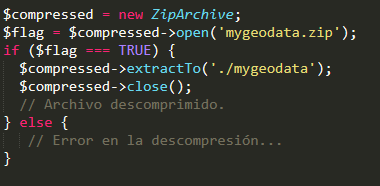
\includegraphics[width=0.7\textwidth]{zip.PNG}
	\caption{Descompresión del \textit{zip} generado por MyGeodata.}\label{fig:zip.PNG}
\end{figure}
\FloatBarrier

\subsection{Añadir fecha y hora a los documentos}
Se planteaba un problema, al subir archivos con el mismo nombre se sobreescribían, para solventarlo se pensó en acompañarlos de la fecha y la hora de forma que cada uno tuviese un nombre único sin tener que forzar al usuarios a renombrarlos ni que se sobresscribieran perdiendo los datos anteriores. Utilizamos la función \textit{date} de PHP y un formato del tipo \textit{dd-mm-yyyy\_h-m-s\_} delante del nombre del fichero.
\imagen{fechas.PNG}{Documentos con el día y la fecha en el título.}

\subsection{Exportar imagen del mapa mostrado y Geolocalización}
Para que el usuario se pueda llevar una instantánea del mapa generado con la ruta, se ha incluido un botón que habilita la descarga de una imagen. Se ha conseguido habilitando el \textit{buffer} de lo dibujado \textit{preserveDrawingBuffer:true} y recuperándolo más tarde cuando demos al botón llamando a \textit{getCanvas()} \cite{descargaimagen}

De igual forma se añadió otro botón para centrar el mapa basándose en tu posición actual. Para ello, se requiere el permiso por parte del navegador y en última estancia del usuario, para poder acceder a tu posición.
\imagen{botones.PNG}{Código que habilita los botones de control, la descarga del mapa y el centrarlo en tu posición.}

\subsection{Añadir una plantilla HTML}
Una vez que la aplicación era funcional, era hora de dotarla de una interfaz agradable al usuario, se utilizó una plantilla basada en \textit{Bootstrap} \cite{plantilla} para la página de inicio, que tras una serie de cambios como: imagen de fondo, textos, imágenes y crear los botones de subida de los archivos, quedó finalizada. Cabe destacar que botones como: ``Iniciar sesión'', ``About'', ``Contact'', ``Terms of Use'', ``Privacy Policy'', los de las redes sociales o el formulario del \textit{email} no se han implementado, pero se han dejado por estética y como línea de mejora de futuro. La página a la que da acceso tras la subida de los ficheros carece de plantilla pues se muestra el mapa a lo largo de la pantalla y contiene 3 botones.
\imagen{pagina.PNG}{Página de inicio con los botones de subida del archivo.}

\subsection{Despliegue de la aplicación}
Para que se pudiera probar la herramienta se necesitaba una placa de desarrollo correctamente programada, o una ruta previamente registrada y una página web. Pensamos que \textit{hostear} la página sería una buena opción, sin embargo finalmente no fue la medida adoptada por diversos motivos. En dominios como \textit{x10hosting} , \textit{5gbfree}, \textit{000webhost} que presentaban una buena oferta gratuita de navegación y número de páginas máximas alojadas, tenían la limitación de no ofrecer Python de forma gratuita, con lo cual no se podía ejecutar la conversión. También se probó en ``GitHub Pages'' arrojando el mensaje ``405 not allowed'' al tratar de ejecutar el código en Python y finalmente tampoco fue posible en \textit{OpenShift} ni \textit{Heroku}. 

Optamos por realizar nuestro despliegue sobre una máquina virtual de Windows 7 limpia que se incluirá en la entrega. Se instaló XAMPP y Python y se configuró correctamente para el correcto funcionamiento.

\subsection{Activación/desactivación por acelerómetro}
Más adelante retomamos una actividad pendiente, que el registro de los datos en la tarjeta microSD dependiera del movimiento con el fin de no almacenar coordenadas de forma repetitiva, por ejemplo en un semáforo. Lo primero fue calibrar el acelerómetro, suponiendo una fuerza de 0G en los ejes 'x' e 'y' y 1G en el eje 'z' proveniente de la gravedad de la tierra, mediante los métodos \textit{FX1\_CalibrateX1g()}, \textit{FX1\_CalibrateY1g()} y \textit{FX1\_CalibrateZ1g()} respectivamente. Más tarde, pusimos como condición que si no se sobrepasaba una fuerza, que establecimos como la mínima para evitar errores producidos por microvibraciones, no se escribiera en la tarjeta microSD.
\imagen{codigoacelerometro.PNG}{Código encargado que calibrar el acelerómetro y capturar los valores de los ejes.}

\subsection{Excepciones PHP}
Por último decidimos crear excepciones para tratar de capturar cualquier error que pudiera surgir en la interfaz. Comprobamos que solo se pudieran subir archivos con extensión txt, que son los que genera la placa, que se moviera a la carpeta ``subidas'' correctamente, que contuviera mensajes NMEA en su interior y que el archivo se convirtiese a GeoJSON sin errores.
\imagen{excepciones.PNG}{Excepción en PHP que comprueba que el archivo subido sea de texto.}

\subsection{Problemas encontrados en el desarrollo}
En este apartado explicaremos algunas cuestiones que nos han provocado retrasos y que detallaremos a continuación por si pudiera servir de ayuda en un futuro.

\subsubsection{La placa deja de funcionar}
En algunas ocasiones es probable que la placa deje de funcionar en el modo de \textit{debugueo} OpenSDA y solo se encienda la luz naranja de corriente. Para solventar esto es necesario enchufar la placa al ordenador mientras se aprieta el botón de \textit{reset} de forma que podamos acceder al \textit{bootloader} y allí pegar el archivo OpenSDA\_V2.bin que se proporciona con el proyecto.

\subsubsection{Comunicación del módulo GPS con la placa}
El módulo GPS tiene un interruptor, para que el envío de datos se produzca de forma satisfactoria debe estar posicionado en ``Soft Serial'' y no en la posición ``Direct''.

\subsubsection{Kinetis no ejecuta los cambios que hemos hecho}
En ciertos momentos nos hemos encontrado con que Kinetis no acometía los cambios que se le había hecho al proyecto, para este problema no hemos encontrado una solución al respecto y la única ha sido reiniciar el programa.

\subsubsection{Cómo copiar y pegar proyectos en Kinetis}
Para poder hacer una copia de tu proyecto y así poder hacer modificaciones sin alterar el original debes hacer antes unos pasos previos:
\begin{itemize}
\tightlist
\item
	Al crear el proyecto evita la opción de que haya archivos enlazados y creálo \textit{standalone} para que los proyectos no compartan archivos y sean independientes.
\item
	Dentro de Project>Properties>C/C++ Build>Settings>Build Artifact>Artifact name asegúrate de poner \${ProjectName} de forma que no referencie al nombre del primer proyecto cuando vaya a ser copiado.
\item
	Evita rutas absolutas dentro de Project>Properties>C/C++ Build> Settings>Tool Settings>Include paths y usa relativas.
\item
	Es una buena idea deshacernos de todo el residuo que pueda haber dejado el proyecto padre, para ello Project>Clean
\end{itemize}
Guía extraída de: \href{https://mcuoneclipse.com/2017/02/18/tips-for-making-copy-of-eclipse-cdt-projects-easier/#more-20572}{\texttt{https://mcuoneclipse.com/2017/02/18/tips-for-making...}}

\subsubsection{Aumentar velocidad de compilación}
Es común que tengas que compilar cada poco tiempo, con el objetivo de reducir el tiempo de espera, es buena idea activar la construcción de código de forma paralela, para ello ve a Project>Properties>C/C++Build>Behavior>Enable Parallel Build y selecciona el máximo que permita tu ordenador.
\capitulo{6}{Trabajos relacionados}

Vamos a hacer un pequeño resumen de las mejores herramientas ya existentes que realizan algo muy similar al proyecto aquí expuesto.

\section{Cronología en Google Maps}
Sin duda para mí, la cronología de Google \cite{cronologia} es la reina indiscutible en este apartado. Se trata de un recolector profesional de ubicaciones, que incluso pausándolo, recolecta tu posición si por ejemplo tienes activado la \textit{Actividad en la Web y en Aplicaciones} (algo que viene por defecto) para personalizar los resultados de tu búsqueda, en función de tu posición o si haces una foto, para añadir la posición donde fue tomada.
Además añade en tu ruta establecimientos visitados, tiempo de visita y no tiene miedo a pronosticar dónde vives o dónde está tu trabajo, gracias a sus algoritmos.

Cuenta con una interfaz muy simple, accesible tanto desde el ordenador como a través de la aplicación móvil de Google Maps, que te permite ver tu recorrido a lo largo de un día cualquiera, gracias a la antena GPS que incorpora tu dispositivo.
Con unos conocimientos avanzados sí se podría desactivar por completo, se puede editar alguna entrada específica o incluso borrarla y por supuesto, es privada.
Descompresión del \textit{zip} generado por MyGeodata.
\begin{figure}[!h]
	\centering
	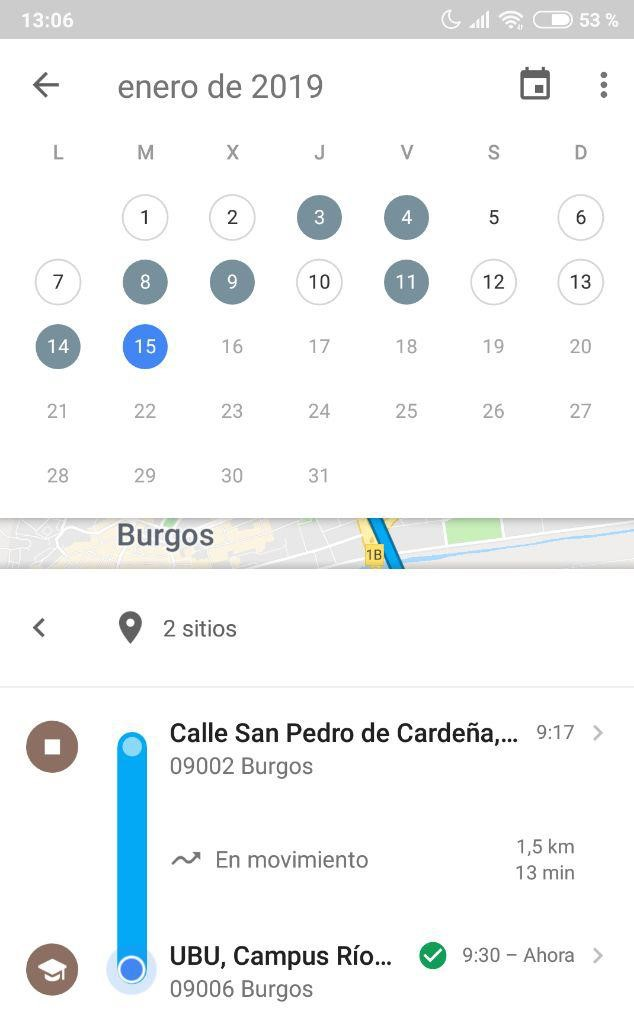
\includegraphics[width=0.4\textwidth]{cronologia.PNG}
	\caption{Se muestran todos los trayectos que se realicen en el día.}\label{fig:cronologia.PNG}
\end{figure}
\FloatBarrier
\begin{figure}[!h]
	\centering
	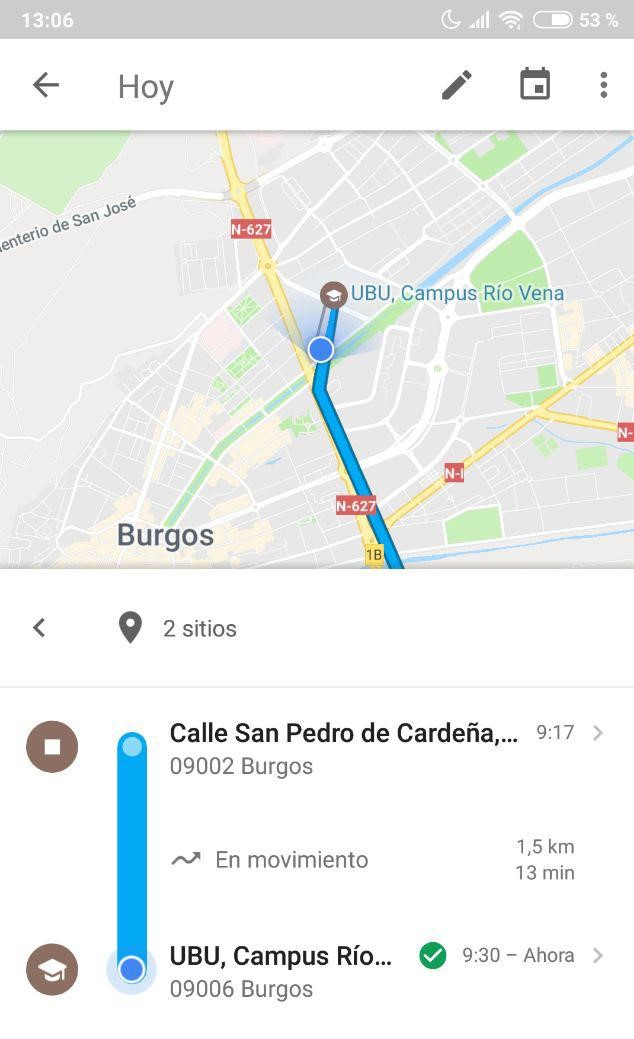
\includegraphics[width=0.4\textwidth]{cronologia2.PNG}
	\caption{Se puede seleccionar cualquier día, desde que tenga datos.}\label{fig:cronologia2.PNG}
\end{figure}
\FloatBarrier

\section{Endomondo}
Endomondo \cite{endomondo} es una aplicación móvil diseñada especificamente para deportistas. Si bien, aparte de recoger la ruta aporta otras muchas opciones y características, realiza la captura de datos de forma correcta gracias al GPS integrado del móvil, pero a diferencia de la anterior, en este caso, tú marcas cuando empieza a registrar tu ruta. Al final de la misma te dice kilómetros recorridos, tiempo invertido, velocidad media, etc.

Cuenta con la posibilidad de crear grupos entre amigos para poder retarles en una misma ruta y así poder comparar tiempos de forma directa a través de la aplicación.
Destaca su amplia compatibilidad con otros dispositivos y cuentas (Garmin Connect, Polar Flow, TomTom MySports o Fitbit) para sumar funcionalidades a la aplicación.

\section{Strava}
Otra aplicación diseñada directamente para el público más deportista, Strava \cite{strava} es considerada la red social de los \textit{runners}, altamente compatible con los pulsómetros más avanzados del mercado, permite una alta interacción entre los usuarios pudiendo ver las rutas de otros y sus estadísticas.

\section{Relive}
La última a comparar Relive \cite{relive}, a pesar de recoger la ruta como los dos anteriores, de forma tradicional y manual, cuenta con algo diferencial, y es la forma en la que es capaz de representar los mapas. Se muestran en forma de vídeo 3D, recreando la ruta por donde has ido pasando e incluyendo fotos y vídeos que hayas hecho por el camino si así lo deseas.
\begin{figure}[!h]
	\centering
	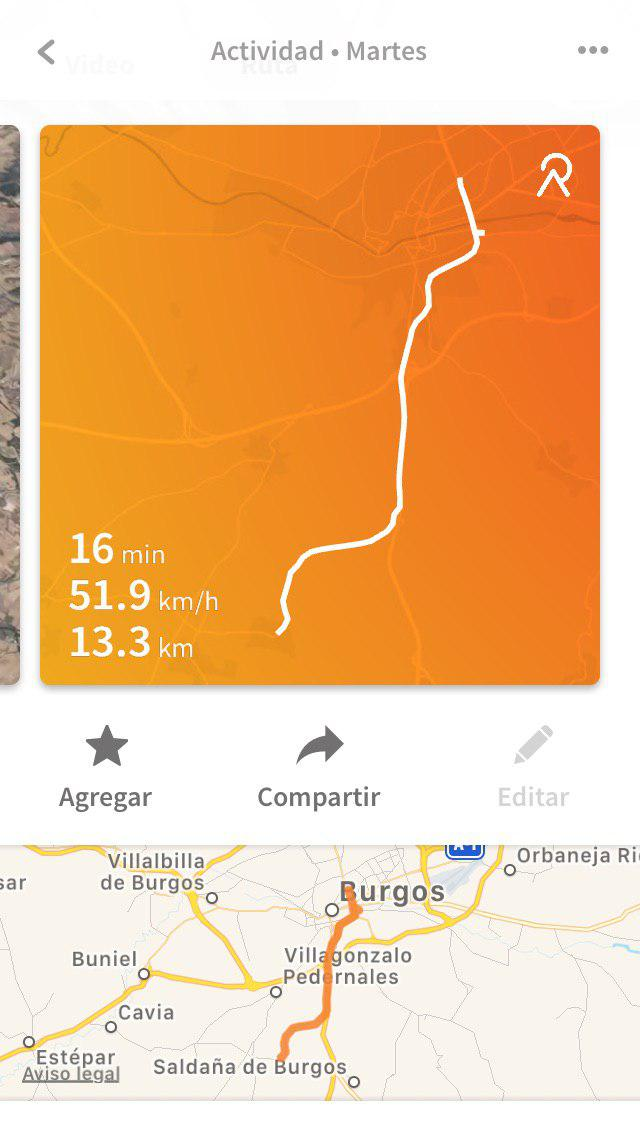
\includegraphics[width=0.4\textwidth]{relive.PNG}
	\caption{Ruta completa tradicional realizada en 2D.}\label{fig:relive.PNG}
\end{figure}
\FloatBarrier
\imagen{relive2.PNG}{Vídeo en 3D recorriendo todos los puntos por los que se ha pasado.}

\section{Conclusión}
Como comentario adicional a todas estas aplicaciones móviles cabe destacar que en mi caso no dispongo de un smartphone, se trata de un registrador de bajo costo, no asociado a ningún terminal móvil y que además almacena las posiciones en una tarjeta microSD. Las aplicaciones finales de este dispositivo podrían ser otras muy diferentes como poder acoplarlo en un coche o en una bici y tener un registro de rutas.



\capitulo{7}{Conclusiones y Líneas de trabajo futuras}

%Todo proyecto debe incluir las conclusiones que se derivan de su desarrollo. Éstas pueden ser de diferente índole, dependiendo de %la tipología del proyecto, pero normalmente van a estar presentes un conjunto de conclusiones relacionadas con los resultados del %proyecto y un conjunto de conclusiones técnicas. 
%Además, resulta muy útil realizar un informe crítico indicando cómo se puede mejorar el proyecto, o cómo se puede continuar %trabajando en la línea del proyecto realizado. 

\section{Conclusiones}
Una vez concluido el trabajo de fin de grado, podría decir que he aprendido más de lo esperado en un primer momento, sobre todo por el tipo de trabajo escogido, tan centrado en los sistemas de posicionamiento y en los sistemas embebidos.

El resultado (al margen de la captura de datos que se da por finalizada), es una interfaz básica, sin pretensiones de ser una herramienta completamente finalizada y con muchas líneas de trabajo futuras, pero con una buena base ya realizada, que agilice su crecimiento y multiplique sus opciones en poco tiempo.

He aprendido mucho sobre los sistemas empotrados, su versatilidad y su gran utilidad a bajo costo. También he aprendido lenguajes nuevos para mi como PHP, herramientas como XAMPP, Termite, Kinetis, Mapbox, MyGeodata o LaTeX y la importancia de las API. He  reforzado mis conocimientos en C, HTML y sistemas en tiempo real y he profundizado sobre el hecho de realizar una página de forma local para luego poder subirla a un hosting.

He alcanzado un nivel de entendimiento sobre posicionamiento GPS, que me permite comprender de una forma más clara cómo funcionan todos los GPS que nos acompañan en el día a día y lo importantes que llegan a ser, en actividades tan diferentes como operaciones de rescate o bancarias.

La organización en un proyecto de esta envergadura es primordial, de forma que planificarme y utilizar una herramienta de gestión como es GitHub, ha formado parte de mi día a día estos últimos meses y, a pesar de que requiere tiempo, finalmente quedan muy bien expuestas todas las fases por las que se ha ido pasando, más si se revisan las diferentes \textit{issues} y \textit{milestones}.


\section{Líneas de trabajo futuras}
\begin{itemize}
	\item
    Permitir la subida múltiple de ficheros.
    \item
    Crear un login de acceso.
    \item
    Crear una base de datos con todos los archivos subidos.
    \item
    Poder acceder a los archivos subidos y mostrar el que se desee.
    \item
    Añadir otros idiomas a la página.
    \item
    Implementar los botones de la interfaz que carecen de funcionalidad.
    \item
    Incluir gráficos y estadísticas.
    \item
    Cambiar la API de pago por otra gratuita o un hacer un parser que convierta los ficheros.
    \item
    Dotar a la placa de conexión a Internet para poder mostrar la ruta en tiempo real.
\end{itemize}


\bibliographystyle{plain}
\bibliography{bibliografia}

\end{document}
